\section{Técnica de evaluación de fiabilidad}
La evaluación de la fiabilidad es de suma importancia para el desarrollo de sistemas críticos, ya
que permite identificar que aspectos del comportamiento del sistema juega un papel importante
\citep{FTDesign}.

\begin{enumerate}
 \item Modelado de un sistema en la fase de diseño.
 \item Aseguramiento del sistema en la fases finales de desarrollo (testing).
\end{enumerate}

La evaulación de la fiabilidad tiene dos aspectos. En primer lugar se tiene una \textit{evaluación
cualitativa} que permite identificar, clasificar y medir modos de fallas, o eventos combinacionales
que puedan provocar una falla. El otro aspecto es la \textit{evaluación cuantitativa}, la cual
permite evaluar en términos de probabilidad los atributos de la fiabilidad
(Sección \ref{sec:atributos_de_la_fiabilidad}), disponibilidad, seguridad.

\section{Medidas comunes de fiabilidad}
Las medidas de fiabilidad más comunes son las siguientes: failure rate, tiempo medio a la falla,
tiempo medio de reparación y tiempo medio entre fallas.

\subsection{Failure rate}
Failure rate $\lambda$ es el número esperardo de fallas por unidad de tiemp \citep{FTDesign}. Es
usual utilizar la dimensión \textit{fallas/horas}.

Generalmente, $\lambda$ se encuentra a nivel de componente. Para conocer el failure rate del
sistema completo, se puede realizar (a groso modo) una sumatoria de los $\lambda$ de los
componentes que integran el sistema. $$\lambda=\sum_{i=1}^{n} \lambda_i$$.

La evolución de $\lambda$ a través del tiempo, no tiene el mismo comportamiento tanto para \ac{HW} como para \ac{SW}
Si se devide el ciclo de vida de un sistema en las siguientes fases: mortalidad prematura (I), vida útil (II), desgaste (II) \citep{FTDesign}
se aprecia, para el caso del \ac{HW}, lo que se denomina \textit{curva de la bañera} la cual puede observarse en la Figura \ref{fig:bathtub_curve}.
En una primera fase, $\lambda$ decrese, ya que a través de los procesos de testing se van descubriendo y resolviendo los errores. Luego se da un periodo de estabilización.
Y al final, el \ac{HW} sufre el paso del tiempo, y se desgasta, aumentando la tasa de fallas.

\begin{figure}[h]
 \centering
 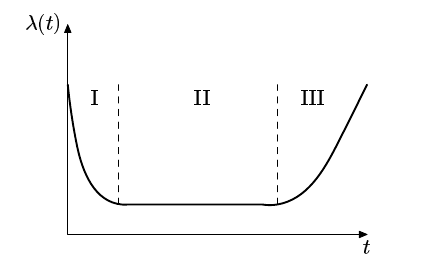
\includegraphics[scale=0.5]{images/Marco_teorico/bathtub_curve.png}
  \caption{Failure rate de HW vs tiempo }
\label{fig:bathtub_curve}
\end{figure}

Para el \ac{SW} es totalmente diferente. En primer lugar cuando se realiza una actualización, se aumenta la complejidad, como así también la probabilidad de fallas,
con ello el failure rate. Otra diferencia sustancia con el \ac{HW} es que el \ac{SW} no se desgasta con el tiempo. En la Figura \ref{fig:Failure_rate_software}
se aprecia $\lamda$ a través de tiempo. Esta curva suele llamarse \texit{curva serrucho}. El failure rate del \ac{SW} decrece en función del tiempo. En estos tipo de sistemas
la tasa de falla depende de varios factores como pueden ser el proceso utilizado en el diseño y codificación, complejidad del \ac{SW}, tamaño del \ac{SW},etc \cite{FTDesign}.

\begin{figure}[h]
 \centering
 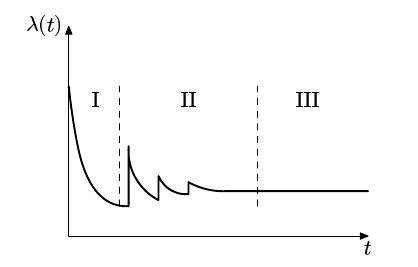
\includegraphics[scale=0.5]{images/Marco_teorico/Failure_rate_software.png}
  \caption{Failure rate SW vs tiempo }
\label{fig:Failure_rate_software}
\end{figure}

A lo largo de la vida de sistema se supone el failure rate $\lambda$ como constante. Por lo tanto la confiabilidad del sistema varía exponencialmente
con respecto al tiempo \cite{FTDesign}: $$R(t) = e^{- \lambda t}$$

Esto se conoce como \textit{ley de la falla exponencial}\cite{FTDesign}. El gráfico de confiabilidad $R(t)$ vs tiempo se muestra en la Figura \ref{fig:failure_rate}.

\begin{figure}[h]
 \centering
 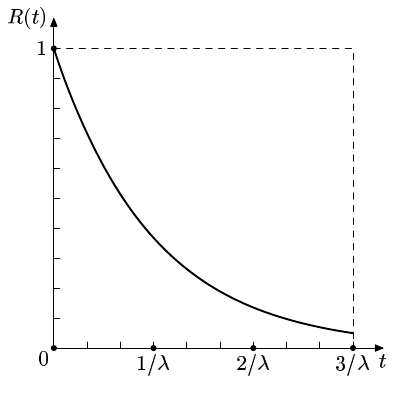
\includegraphics[scale=0.5]{images/Marco_teorico/failure_rate.png.png}
  \caption{Confiabilidad vs tiempo }
\label{fig:failure_rate}
\end{figure}

\subsection{Tiempo medio medio de falla}
\textit{El tiempo medio de falla} (MTTF\footnote{Del inglés, Mean Time To Failure}) de un sistema es el tiempo esperado que transcurra hasta la primera falla que se
detecte en el sistema. En terminos de confiabilidad, MTTF se define de la siguiente manera \cite{FTDesign} $$\int_0^{\infty} R(t) dt$$

\subsection{Tiempo medio de reparación}
\textit{El tiempo medio de reparación}(MTTR\footnote{Del inglés, Mean Time To Repair})de un sistema, es el promedio de tiempo que se requiere para reparar al sistema.
MTTR se especifica en términos de la tasa de reparación $\mu$ \cite{FTDesign}, el cual es el número esperarado de reparaciones por unidad de tiempo: $$MTTR = \frac{1}{\mu}$$

El MTTR depende de los mecanismos de recuperación ante fallas que se utilicen en el sistema, localización del sistema, scheduler de mantenimiento \cite{FTDesign}.
Con esto se puede definir la disponibilidad como sigue: $$A(\infty) = \frac{MTTF}{MTTF+MTTR}$$

\subsection{Tiempo medio entre fallas}
\textit{El tiempo medio entre fallas}(MTBF\footnote{Del inglés, Mean Time Between Failure}) de un sistema es el tiempo promedio entre dos fallas del sistema. $$MTBF = MTTF + MTTR$$

\subsection{Cobertura de fallas}
La cobertura de fallas es la probabilidad  de que el sistema no interrumpirá su actividad cuando una falla se presente. En términos matemáticos la cobertura
de fallas la probabilidad condicional $P(A|B)$. Existen diferentes coberturas de fallas, dependiendo de si se está tratando con detección de fallas, localización de fallas, contención de
fallas o recuperación de fallas \cite{FTDesign}. Siendo $A$ detección, localización, contensión o recuperación de fallas, y $B$ la existencia de fallas.
